\subsection*{PGL: Prior-Guided Local Self-supervised Learning
for 3D Medical Image Segmentation}

% \subsubsection*{Ссылка} \url{https://arxiv.org/abs/2011.12640}
\subsubsection*{Введение}
В данной работе \cite{ann15} предланается self-supervised модель Prior-Guided Local (PGL) 
для сегментации трехмерных медицинских изображений, которая использует изначально
известное расположение между парой позитивных изображений, чтобы выявить местную 
зависимость признаков в одном и том же регионе.
\subsubsection*{Основная идея}
Предложенная модель состоит из модуля аугментации данных для генерации 
представлений изображения и модуля известного двойного пути (prior dual-path module)
для извлечения признаков. Далее конструируется функция потерь местных зависимостей, 
для минимизации различий между каждой парой выявленных признаков. Таким образом, модель
учится захватывать больше структурной информации и больше подходит для решения задачи сегментации, 
чем методы, основанные на выявлении глобальных зависимостей. 
\par 
\textbf{Отличие метода PGL от BYOL} \par
\textit{Bootstrap Your Own Latent (BYOL)} - метод, в котором сеть 
обучается онлайн на представлениях изображений для того, чтобы предсказать вид
следующего представления. BYOL фокусируется на изучении глобальных зависимостей между 
парой представлений, в то время как PGL использует априорную информацию о
взаимном расположении двух представлений, чтобы извлечь локальные зависимости в одинаковых регионах.




\begin{minipage}{1.0\linewidth}
    \begin{center}
        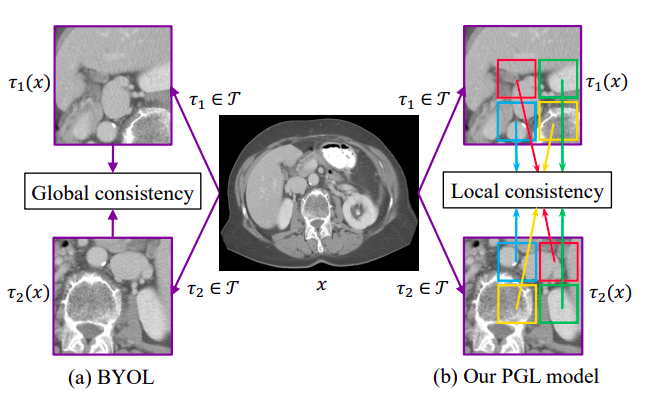
\includegraphics[scale=0.5]{ann15_byol.png} \\
        \captionof{figure}{\scriptsize{BYOL и PGL}}
    \end{center}
\end{minipage}
\\
\begin{minipage}{1.0\linewidth}
    \begin{center}
        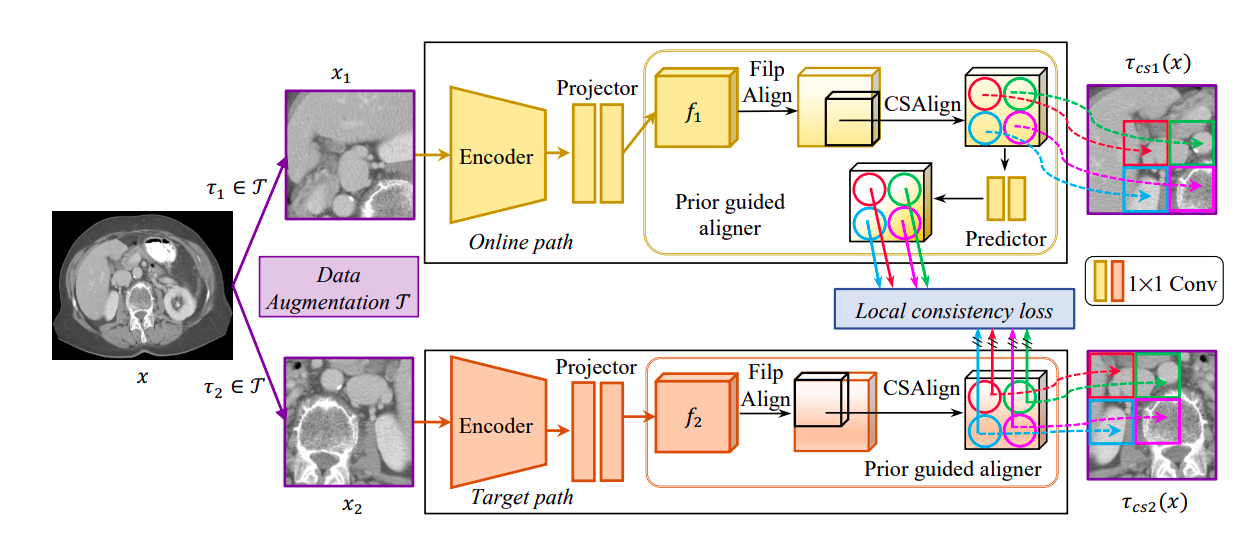
\includegraphics[scale=0.35]{ann15_arch.png} \\
        \captionof{figure}{\scriptsize{Архитектура PGL}}
    \end{center}
\end{minipage}
\subsubsection*{Данные}
Liver,Spleen,KiTS, BCV из Medical Segmentation
Decathlon (MSD) соревнования, RibFac датасет.
\subsubsection*{Результаты}
Производительность baseline сети с использованием случайной инициализации или одной из трех 
стратегий предобучения: Models Genesis (MG), BYOL и  PGL на датасете BCV:

\newpage

{\small 
\begin{center}
    \captionof{table}{Результаты предсказания моделей на датасете BCV. Ave - 
    средний результат сегментации 13 органов.}
    \resizebox{\columnwidth}{!}{
    \begin{tabular}{|c|c|c|c|c|c|c|c|c|c|c|c|c|c|c|c|}
    \hline
    \multicolumn{2}{|c|}{}                                 & \multicolumn{13}{c|}{Organs}                                                                           &                       \\ \cline{3-15}
    \multicolumn{2}{|c|}{\multirow{-2}{*}{Methods}}        & Sp    & RK    & LK    & Gb    & Es    & Li    & St    & Aorta & IVC   & PSV & Pa    & RAG   & LAG   & \multirow{-2}{*}{Ave} \\ \hline
    \rowcolor[HTML]{F8EAE9} 
    \cellcolor[HTML]{F8EAE9}                       & Random Init & 94.01 & 92.97 & 92.15 & 51.98 & 71.85 & 94.82 & 77.74 & 87.47 & 84.85 & 70.91  & 74.12 & 62.27 & 67.30  & 78.65                 \\ \cline{2-16} 
    \rowcolor[HTML]{F8EAE9} 
    \cellcolor[HTML]{F8EAE9}                       & MG  & 94.92 & 93.03 & 91.87 & 59.80 & 71.28 & 95.27 & 80.88 & 87.92 & 85.34 & 71.95  & 75.88 & 63.70 & 67.77 & 79.97                 \\ \cline{2-16} 
    \rowcolor[HTML]{F8EAE9} 
    \cellcolor[HTML]{F8EAE9}                       & BYOL& 95.04 & 93.53 & 92.55 & 59.70 & 70.98 & 95.35 & 80.69 & 88.37 & 85.36 & 71.93  & 75.95 & 63.71 & 68.27 & 80.11                 \\ \cline{2-16} 
    \rowcolor[HTML]{F8EAE9} 
    \multirow{-4}{*}{\cellcolor[HTML]{F8EAE9}Dice~$\uparrow$} & \textbf{PGL(Ours)} & \textbf{95.46} & \textbf{93.54} & \textbf{92.62} & \textbf{59.91} & \textbf{72.59} & \textbf{96.14} & \textbf{81.99} & \textbf{89.20} & \textbf{86.49} & \textbf{72.50}  & \textbf{77.00} & \textbf{63.85} & \textbf{69.75} & \textbf{80.85}                 \\ \hline
    \rowcolor[HTML]{EBECFE} 
    \cellcolor[HTML]{EBECFE}                       & Random Init & 88.87 & 86.95 & 85.76 & 40.97 & 57.12 & 90.51 & 65.87 & 78.65 & 73.95 & 55.42  & 59.48 & 46.95 & 51.43 & 67.84                 \\ \cline{2-16} 
    \rowcolor[HTML]{EBECFE} 
    \cellcolor[HTML]{EBECFE}                       & MG & 90.44 & 87.06 & 85.19 & \textbf{47.86} & 56.52 & 91.28 & 69.98 & 79.07 & 74.68 & 56.74  & 61.60 & 48.31 & 51.8  & 69.27                 \\ \cline{2-16} 
    \rowcolor[HTML]{EBECFE} 
    \cellcolor[HTML]{EBECFE}                       & BYOL& 90.63 & 87.89 & 86.42 & 47.73 & 56.30 & 91.43 & 69.71 & 79.74 & 74.72 & 56.70  & 61.69 & 48.06 & 52.31 & 69.49                 \\ \cline{2-16} 
    \rowcolor[HTML]{EBECFE} 
    \multirow{-4}{*}{\cellcolor[HTML]{EBECFE}IoU~$\uparrow$}  & \textbf{PGL(Ours)} & \textbf{91.35} & \textbf{87.93} & \textbf{86.50} & 47.72 & \textbf{58.19} & \textbf{92.63} & \textbf{71.84} & \textbf{80.90} & \textbf{76.38} & \textbf{57.37}  & \textbf{63.00} & \textbf{48.32} & \textbf{54.16} & \textbf{70.48}                 \\ \hline
    \rowcolor[HTML]{FEFED6} 
    \cellcolor[HTML]{FEFED6}                       & Random Init & 38.31 & 2.06  & 2.54  & 51.75 & 8.83  & 3.64  & 48.28 & 26.92 & 6.12  & 16.73  & 14.66 & 5.22  & 3.82  & 17.61                 \\ \cline{2-16} 
    \rowcolor[HTML]{FEFED6} 
    \cellcolor[HTML]{FEFED6}                       & MG & 4.43  & 2.07  & 24.89 & 12.69 & 7.65  & 3.24  & 20.77 & 26.20 & 5.20  & \textbf{8.61}   & 6.02  & 5.31  & 4.44  & 10.12                 \\ \cline{2-16} 
    \rowcolor[HTML]{FEFED6} 
    \cellcolor[HTML]{FEFED6}                       & BYOL& 3.46  & 1.92  & \textbf{2.45}  & 25.96 & 20.41 & 3.11  & 22.61 & 17.45 & 5.20  & 16.36  & 5.94  & \textbf{4.52}  & 4.46  & 10.30                 \\ \cline{2-16} 
    \rowcolor[HTML]{FEFED6} 
    \multirow{-4}{*}{\cellcolor[HTML]{FEFED6}HD~$\downarrow$} & \textbf{PGL(Ours)} & \textbf{2.50}  & \textbf{1.83}  & 2.47  & \textbf{11.52} & \textbf{7.18}  & \textbf{2.52}  & \textbf{12.45} & \textbf{6.23}  & \textbf{4.77}  & 13.85  & \textbf{6.00}  & 4.75  & \textbf{3.56}  & \textbf{6.13}                  \\ \hline
    \end{tabular}
    }
\end{center}
}
% {\small
% \captionof{table}{\scriptsize{Производительность PGL модели с различными пространственными 
% трансформациями на датасете Liver. Ave - 
% средний результат сегментации печени и опухоли печени.}}
% \begin{center}
%     \begin{tabular}{c|c|c|c|c|c}
%     \hline
%     \multicolumn{2}{c|}{}         & \begin{tabular}[c]{@{}c@{}}Random \\ {Init}\end{tabular}  & \begin{tabular}[c]{@{}c@{}}Models \\ {Genesis}\end{tabular}    & \begin{tabular}[c]{@{}c@{}}BYOL \\ \end{tabular}  & \begin{tabular}[c]{@{}c@{}}\textbf{PGL} \\ {\textbf{(Ours)}}\end{tabular}  \\ \hline
%     \multirow{3}{*}{Organ} & Dice~$\uparrow$ & 95.73  & 96.00 & 96.29 & \textbf{96.43} \\ \cline{2-6} 
%                            & IoU~$\uparrow$  & 91.94  & 92.45 & 92.92 & \textbf{93.16} \\ \cline{2-6} 
%                            & HD~$\downarrow$ & 7.49   & 4.75  & 5.46  & \textbf{4.72}  \\ \hline
%     \multirow{3}{*}{Tumor} & Dice~$\uparrow$ & 52.20  & 53.47 & 53.34 & \textbf{55.66} \\ \cline{2-6} 
%                            & IoU~$\uparrow$  & 41.64  & 42.91 & 43.25 & \textbf{44.95} \\ \cline{2-6} 
%                            & HD~$\downarrow$ & 29.69  & 29.87 & 32.82 & \textbf{24.01} \\ \hline
%     \multirow{3}{*}{Ave}   & Dice~$\uparrow$ & 73.97 & 74.74 & 74.82 & \textbf{76.05} \\ \cline{2-6} 
%                            & IoU~$\uparrow$  & 66.79  & 67.68 & 68.09 & \textbf{69.06} \\ \cline{2-6} 
%                            & HD~$\downarrow$ & 18.59  & 17.31 & 19.14 & \textbf{14.37} \\ \hline
    
%     \end{tabular}
% \end{center}
% }



% \begin{minipage}{0.49\linewidth}
%     \begin{center}
%         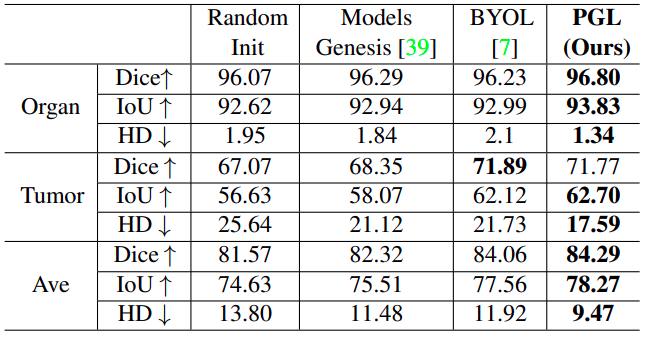
\includegraphics[scale=0.35]{ann15_res3.png} \\
%         % \caption{\scriptsize{Производительность PGL модели с 
%         % различными пространственными 
%         % трансформациями на датасете KiTS. Ave - 
%         % средний результат сегментации почек и опухолей почек.}}
%     \end{center}
    
% \end{minipage} 


\subsubsection*{Заключение}
Были проведены масшатбные эксперименты на четырех КТ датасетах, которые включали в себя 
11 органов и два вида опухолей. Результаты показали, что использование PGL для инифиализации 
сети для сегментации позволяет сильно улучшить производительность сети, также показано 
превосходство предложенной модели PGL над моделью BYOL.